\xchapter{Plataforma e metodologia}{}\label{cap3}

Esta seção cobrirá as especificações do ambiente usado para realizar as medições e a metodologia utilizada. Serão apresentados alguns exemplos de soluções tecnológicas para tornar o sistema Linux um sistema operacional de tempo real. Também serão apresentados os componentes da plataforma Raspberry Pi e o módulo INTSight usado para realizar as medições.

\section{Soluções de SOTR Linux}

Existem várias maneiras de tornar o Linux um sistema operacional de tempo real, mas existem duas maneiras principais de atingir esse objetivo. A primeira maneira é alterar a configuração do kernel durante a compilação, permitindo que as tarefas do kernel sejam preemptadas também. A segunda maneira é usar um nanokernel para intermediar o kernel com o hardware.

Xenomai é um patch que usa a estratégia de nanokernel. Os nanokernels agem como uma camada extra de abstração entre o hardware e o kernel. Ele lida com interrupções de hardware e as define como interrupções para aplicativos em tempo real ou interrupções não críticas. Se for uma interrupção de uma tarefa de tempo real, ele interrompe o kernel para que a tarefa seja executada imediatamente. Caso contrário, enfileira a tarefa para executar em outro momento \cite{Xenomai2005}.

O patch Preempt-RT é o patch de tempo real padrão para o Raspberry Pi e vários outros casos em que o Linux é usado. Este patch torna o kernel completamente preemptivo para diminuir a latência de interrupção. O desenvolvimento é liderado por Ingo Molnar e tem a participação de muitos desenvolvedores em todo o mundo \cite{McKenney2005, Molnar2016}. É o patch que foi usado para as medições neste trabalho e será descrito agora.

\subsection{Preempt-RT}\label{Preempt-RT}

As interrupções são capazes de interromper as tarefas que são executadas no espaço do usuário, mas às vezes as tarefas do kernel já levam um tempo considerável, portanto pode ser necessário interromper essas tarefas e dar lugar a uma tarefa de maior prioridade, como o tratamento de uma interrupção. Interromper uma tarefa para executar outra, e depois poder retornar a tarefa anterior, é chamado de preempção. O kernel do Linux tem vários níveis de preempção:

\begin{itemize}
  \item PREEMPT\_NONE: as preempções ocorrem apenas nas tarefas do usuário.
  \item PREEMPT\_VOLUNTARY: algumas partes do kernel tem pontos específicos que permitem a preempção.
  \item CONFIG\_PREEMPT: semelhantes ao PREEMPT\_VOLUNTARY mas com uma região de preempção maior.
  \item PREEMPT\_RT\_FULL: praticamente qualquer seção do kernel pode ser preemptada, exceto algumas partes extremamente críticas.
\end{itemize}

Na figura \ref{grafic:Preempt} podemos ver em vermelho as partes do kernel que não podem ser preemptadas e em verde as partes que podem ser preemptadas para cada modo de configuração.

\begin{figure}[!htb]
\centering
\subfloat[PREEMPT\_NONE]{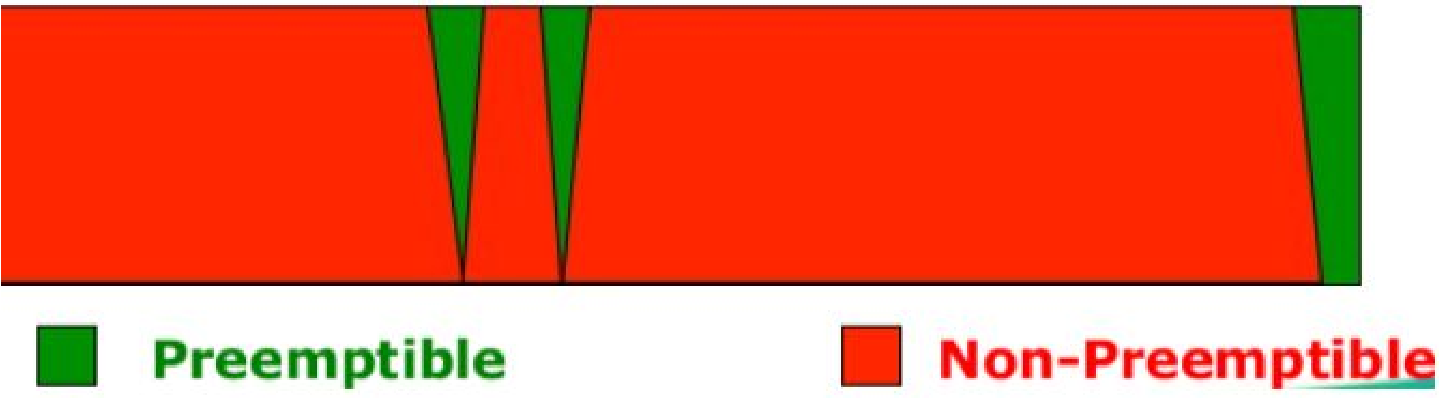
\includegraphics[width = .4\textwidth]{graficos/PREEMPT_NONE.png}}%
\subfloat[PREEMPT\_VOLUNTARY]{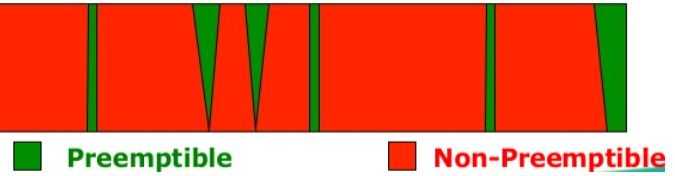
\includegraphics[width = .4\textwidth]{graficos/PREEMPT_VOLUNTARY.png}}\\
\subfloat[CONFIG\_PREEMPT]{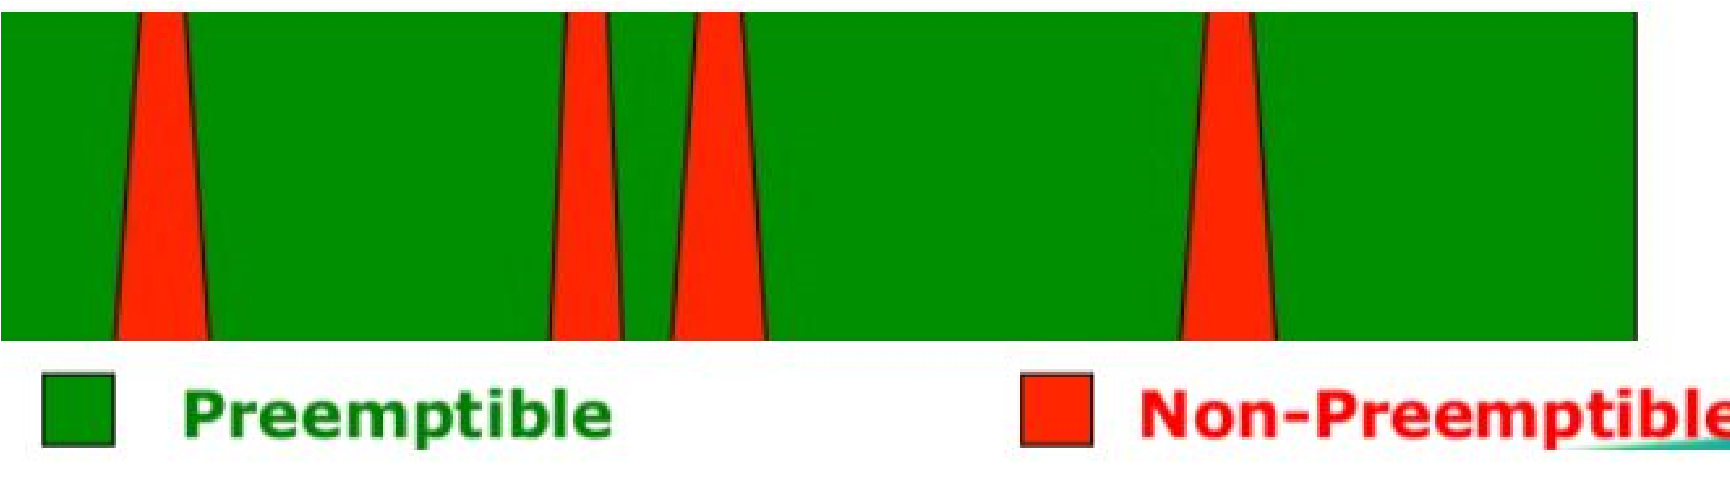
\includegraphics[width = .4\textwidth]{graficos/CONFIG_PREEMPT.png}}%
\subfloat[PREEMPT\_RT\_FULL]{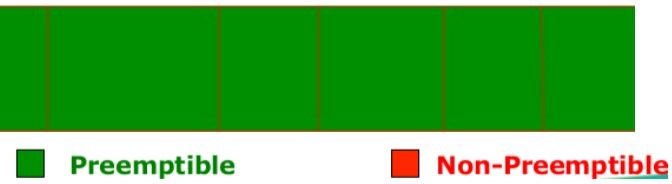
\includegraphics[width = .4\textwidth]{graficos/PREEMPT_RT_FULL.png}} 
\caption{Configurações de preempção no kernel \cite{Huang2017}}
\label{grafic:Preempt}
\end{figure}

O patch Preempt-RT corresponde à configuração PREEMPT\_RT\_FULL. Nele, mesmo algumas seções críticas podem ser preemptadas, portanto, uma tarefa crítica pode acabar sendo movida para outro núcleo durante a execução. Quase todos os tratadores de interrupção são executados no contexto do processo no ambiente Preempt-RT, incluindo o Softirq, que será executado pela thread \textit{ksoftirqd}, permitindo que os tratadores sejam interrompidos. As exceções são a invocação do RCU (read-copy update) e os \textit{timers}, que continuam com o Softirq tradicional.

Quando uma interrupção ocorre, o tratador associado mascara novas interrupções, acorda a thread que vai tratar a interrupção e volta para o código interrompido. Com isso a parte crítica do tratador de interrupção é o mínimo necessário e a latência dessa execução é muito curta e determinística. A thread acordada em algum momento será escalonada de acordo com sua prioridade e a interrupção será tratada. Isso aumenta a capacidade de resposta do kernel, mas também diminui o seu \textit{throughput}, a quantidade de trabalho realizada por tempo.

\section{Raspberry Pi}

Raspberry Pi é um computador completo, do tamanho de um cartão de crédito, com todo o hardware em uma única placa. Tem um preço acessível e é amplamente utilizado para projetos que exigem um computador portátil. Mantido pela Raspberry Pi Foundation \cite{RPF2019}, seu principal objetivo é promover a educação em informática. O primeiro modelo foi lançado em 2012 e se tornou um enorme sucesso.

O modelo usado neste trabalho é o Raspberry Pi 3 Model B. Este modelo possui um processador Broadcom BCM2837 com quatro núcleos, 1,2 GHz de frequência, arquitetura de 64 bits, 1 GB de RAM, acesso WIFI, Bluetooth, entrada Ethernet, 40 pinos de uso geral, 4 entradas USB, saídas de áudio e vídeo, saída HDMI e slot para cartão microSD.

O sistema operacional padrão é o Linux na distribuição Raspbian, uma distribuição baseada no Debian. Qualquer outra distribuição compatível com a arquitetura ARM pode ser usada e o fabricante fornece um utilitário para ajudar na escolha e gravação do sistema operacional em um cartão SD, que será a principal memória de dados do Raspberry Pi.

\begin{figure}[!htb]
    \centering
    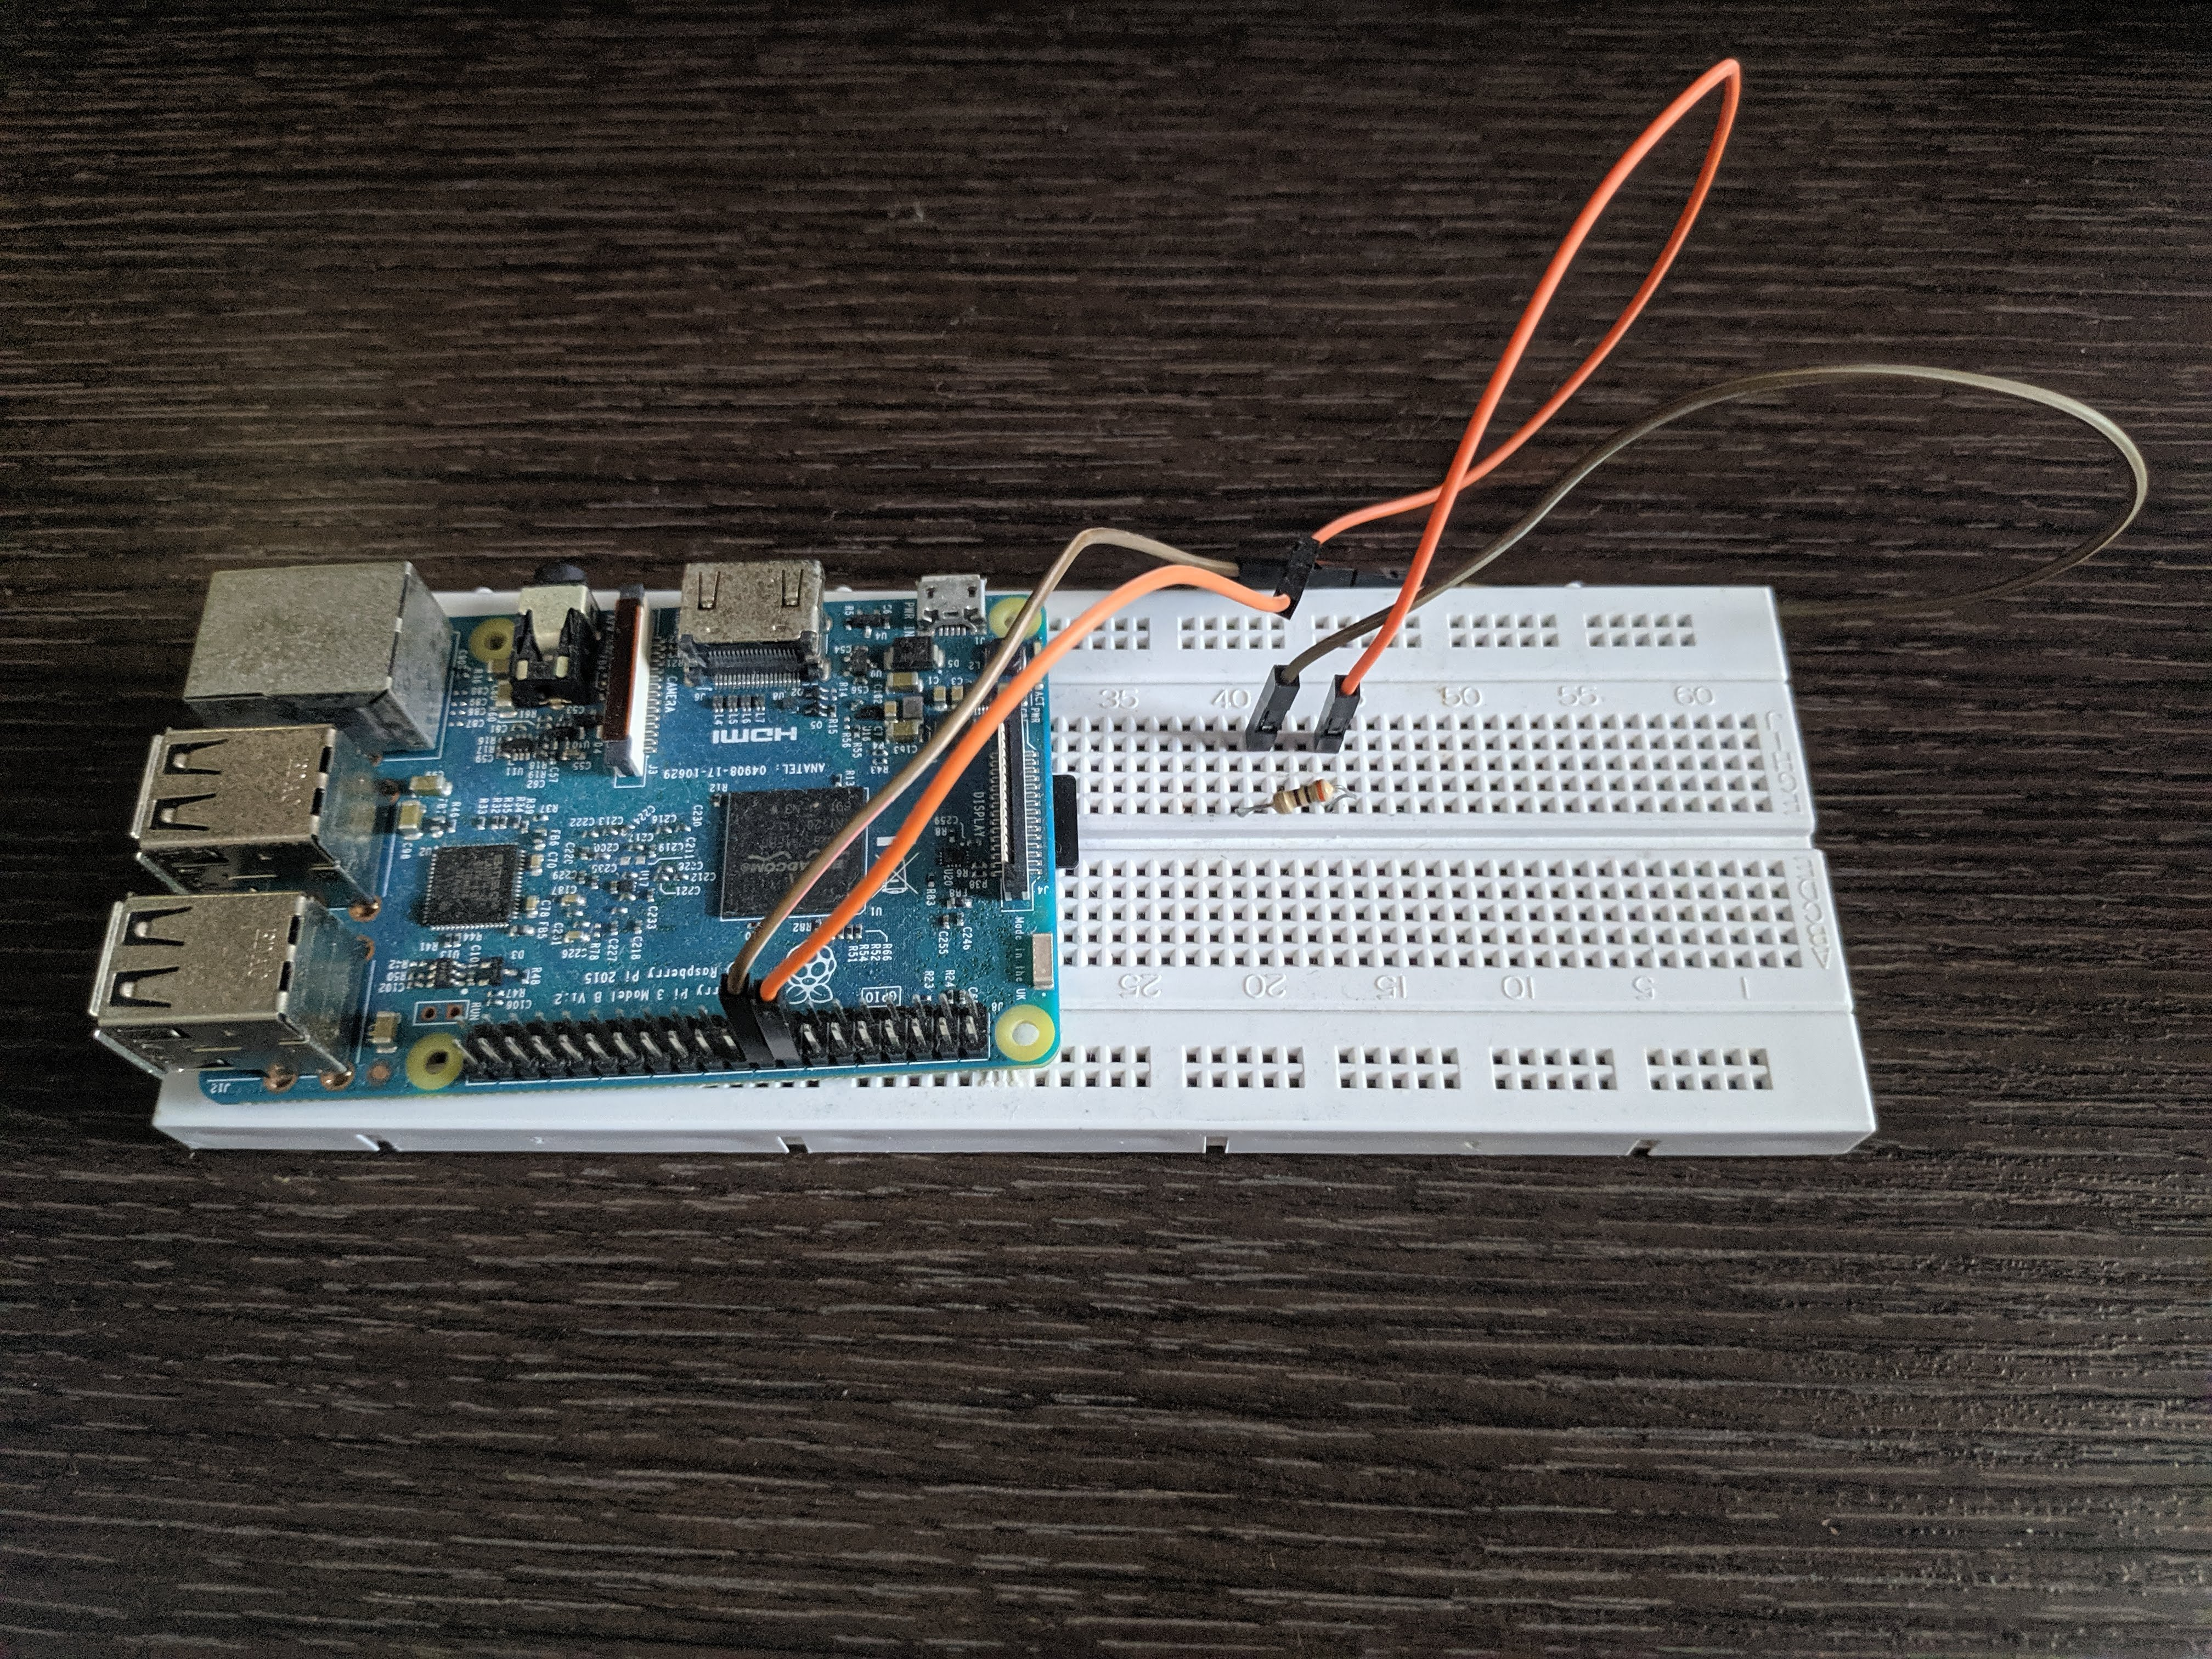
\includegraphics[width=.8\textwidth]{photos/raspberry-photo.jpg}
    \caption{Foto do Raspberry Pi com a montagem feita para as medições}
    \label{foto:Raspberry Pi}
\end{figure}

\section{Módulos INTSpect e INTSight}\label{INTSight}

Em sistemas computacionais complexos, o número de variáveis é tão grande que não há um cálculo que possa ser feito para prever o tempo que uma interrupção leva para ser tratada, pois não basta levar em consideração a especificação de hardware, que geralmente não é aberta para impedir que os segredos industriais sejam expostos aos concorrentes, deve-se também levar em consideração toda a estrutura de software do sistema operacional. Portanto, a realização de medições empíricas é a melhor maneira de avaliar a latência do sistema em sistemas reais. No entanto, fazer essas medições nem sempre é trivial.

Com o exposto no parágrafo anterior em mente, Luis Gerhorst \cite{Gerhorst2018} desenvolveu uma ferramenta para ajudar os desenvolvedores a fazer essas medições e analisar o tempo de resposta. Esta ferramenta foi dividida em 2 módulos: INTSight, que é um módulo do kernel responsável por fazer medições, e INTSpect, que é um módulo para acionar benchmarks no INTSight. 

O INTSight é capaz de medir a latência de interrupção e latência de ativação, suporta vários métodos de medição, gera dados de formato simples a serem analisados posteriormente para medições sem comprometimento e tira fotos do sistema antes das sequências de medição para tornar os resultados facilmente reproduzíveis. O INTSight insere \textit{checkpoints} em várias partes do código do kernel e toda vez que aquele código é executado é realizada uma medição do tempo de execução com o mecanismo especificado e salva em memória. Assim, é possível identificar quando ocorreram trocas de contexto, quando o escalonador foi executado entre outras ações. Os locais no código onde o INTSight faz medições são definidos em tempo de compilação. Isso troca flexibilidade por maior precisão de medição. Uma abordagem com um hardware externo pode trazer resultados mais precisos, mas o INTSight tem a vantagem de ter um custo praticamente nulo com equipamentos, tornando-o uma ferramenta poderosa para fazer testes iniciais antes de se investir em testes mais rigorosos.

O INTSight tem a função de realizar medições de latência de ativação para os vários mecanismos disponíveis no Linux com o mínimo de interferência possível. Na inicialização, o INTSight aloca uma rotina de serviço de interrupção (\textit{ISR - Interrupt Service Routine}) e um tratador para o mecanismo: Softirq, Tasklet ou Workqueue; usado para o teste. Para considerar as variações que ocorrem, o número de medições pode ser definido. No início de cada medição, uma thread coordena a ativação da interrupção usando um mecanismo dependente da plataforma.

O trabalho do INTSight compara vários métodos de medição e seus custos associados. Os métodos de medição analisados pelo INTSight foram o \textit{PMCCNTR} (\textit{Performance Monitors Cycle Count Register}), o \textit{k\_time\_mono\_fast}, o \textit{k\_time} e o \textit{nstimeofday}. O método de medição utilizado foi \textit{k\_time\_mono\_fast}, porque é o segundo método de menor custo dentre os apresentados por \cite{Gerhorst2018}. O método com menor custo para uma plataforma ARM seria usar o \textit{PMCCNTR}, que é um registrador específico capaz de contar o número de pulsos de clock que ocorreram no processador, portanto, lê-los tem o custo de leitura de um registrador. Nas medições feitas para o trabalho do INTSight, foi utilizada uma placa de núcleo único. Conhecendo a frequência de operação do processador, é possível saber o tempo decorrido executando uma conta simples. No Raspberry Pi, no entanto, temos um processador de quatro núcleos e não temos garantia de que o núcleo que lidará com a interrupção seja o mesmo que o acionou. Como cada núcleo tem seu próprio contador, os valores não podem ser comparados. Para continuar com esse método de medição, precisaríamos usar apenas um núcleo Raspberry Pi, desativando os outros ou inserindo outro mecanismo de sincronização. Isso mudaria o comportamento real do processador do Raspberry Pi e resultaria em algo que não é comparável a uma situação de uso real.

Para gerar as interrupções de hardware no Raspberry Pi, foram utilizados os pinos 16 e 18, BCM23 e BCM24, respectivamente. Um dos pinos estava no modo de escrita, enviando um sinal para o outro, definido no modo de leitura. O Raspberry Pi usa 3,3 V em seus pinos digitais e o guia de uso indica que não deve ter uma corrente maior que 16 mA na entrada do pino, portanto, um resistor de \SI{300}{\ohm} foi usado para fazer a conexão entre os pinos.

\begin{figure}[!htb]
\centering
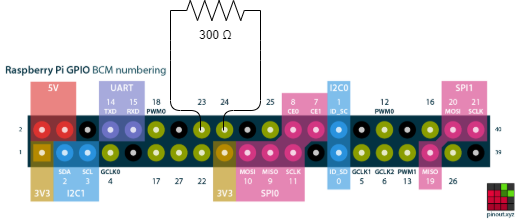
\includegraphics[width = \textwidth]{photos/raspberry-pins.png}
\caption{Esquema da montagem para o teste. Imagem de retirada de \cite{pinout}}
\label{grafic:Preempt}
\end{figure}
